\documentclass[11pt,letterpaper]{article}
%% Coverpage Packs
\usepackage{wallpaper}

%%Query packs
\usepackage[utf8]{inputenc}
\usepackage{amsmath}
\usepackage{amsfonts}
\usepackage{amssymb}
\usepackage{url}
\usepackage{xcolor}
\usepackage{fullpage}
\usepackage{listings}
\usepackage{mathtools}
\usepackage{enumitem}
\usepackage{bm}
\usepackage{fixltx2e}
\usepackage{hyperref}
\usepackage{array}
\usepackage{multirow}
\usepackage{longtable}

\lstset{
	basicstyle=\ttfamily,
	columns=fullflexible,
	breaklines=true,
	postbreak=\mbox{\textcolor{red}{$\hookrightarrow$}\space},
}
\setlength\parindent{24pt}

%%Graphics packs
\usepackage{ulem}
\usepackage{geometry, tikz}
  \usepackage{graphicx}
\usetikzlibrary{shapes,shadows,arrows.meta}
\geometry{
    a4paper,
    total={170mm,257mm},
    left=20mm,right=20mm,
    top=20mm,
}

%%Assumption/Constraint Packs
\usepackage{enumitem}

\title{Comp353 Project Report}
\author{Kai Nicoll-Griffith[40012407], Stephen Prizio[40001739], \\Giovanni Gebran[40018637], Nizar Belhassan[27519443]\\\\\bf{Team kzc353\_4}}

\begin{document}
	
	

	\begin{titlepage}
\iffalse
\tikz[remember picture,overlay] \node[opacity=1.0,inner sep=0pt] at (current page.center){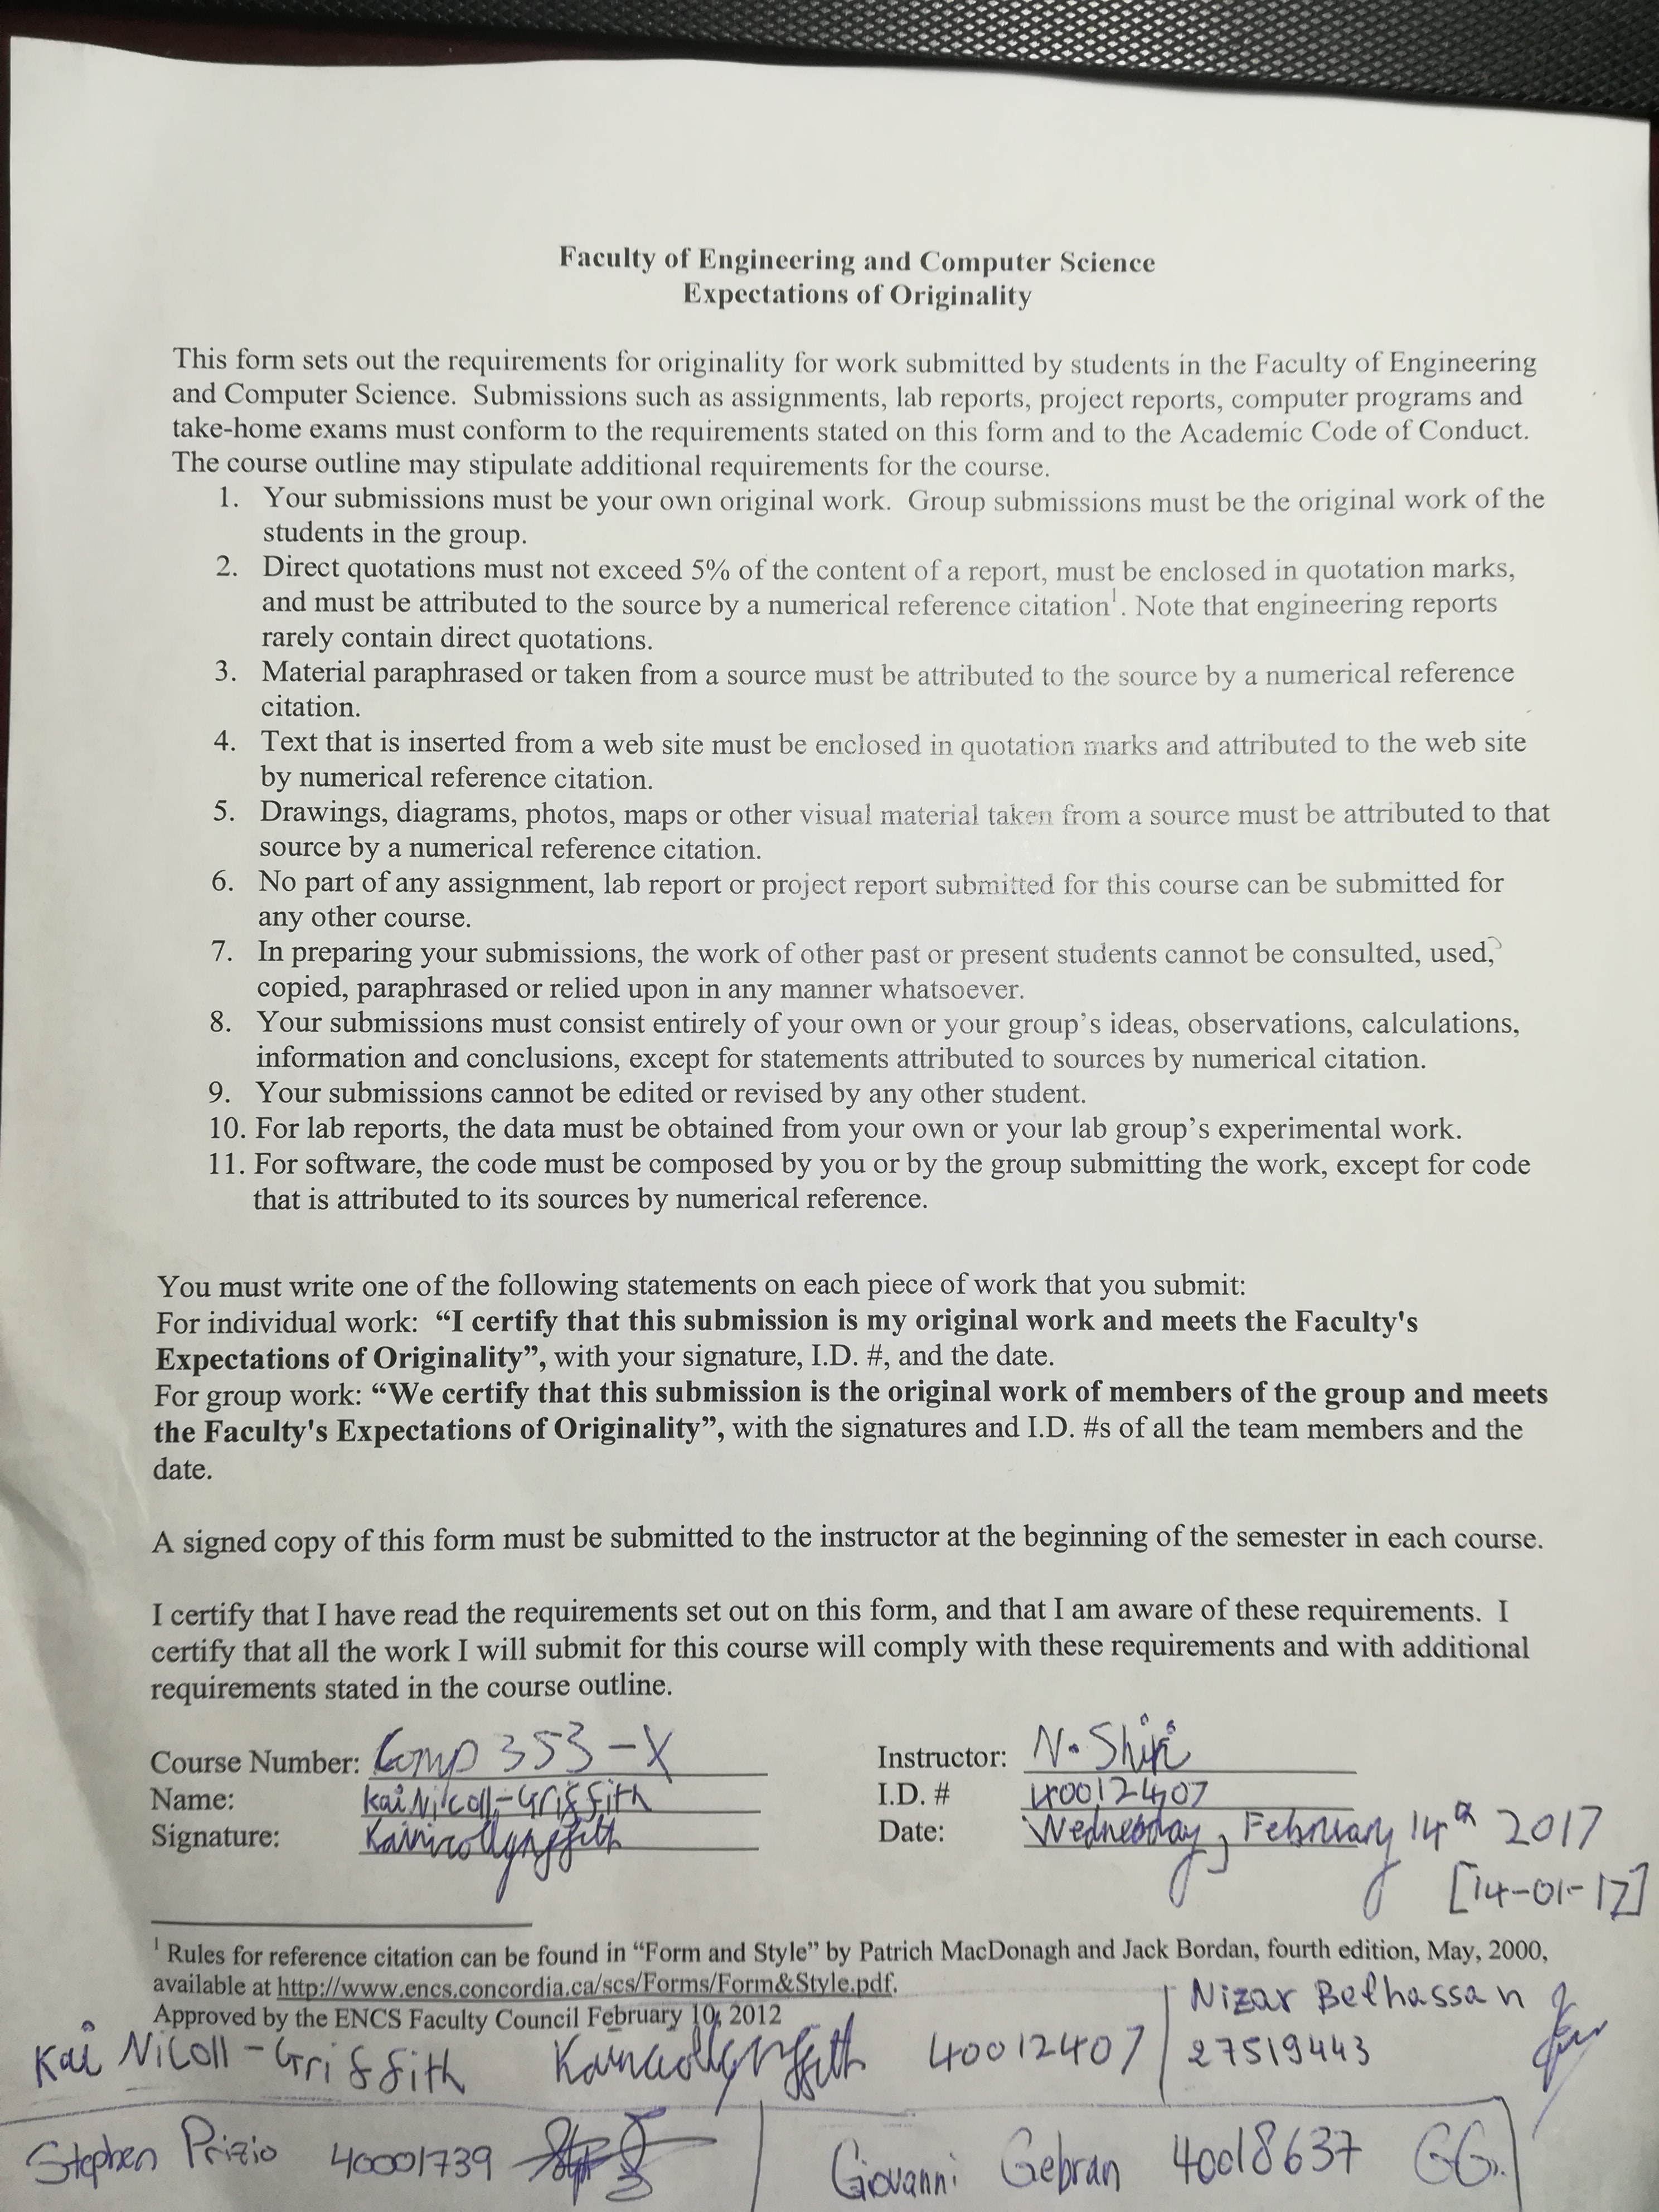
\includegraphics[width=\paperwidth,height=\paperheight]{originality.jpg}};
\fi
\end{titlepage}
	
		\maketitle
		\newcommand{\graphicwidth}{18.5cm}
	\section{Entity Relationship Diagram}
\hspace*{-1.1cm}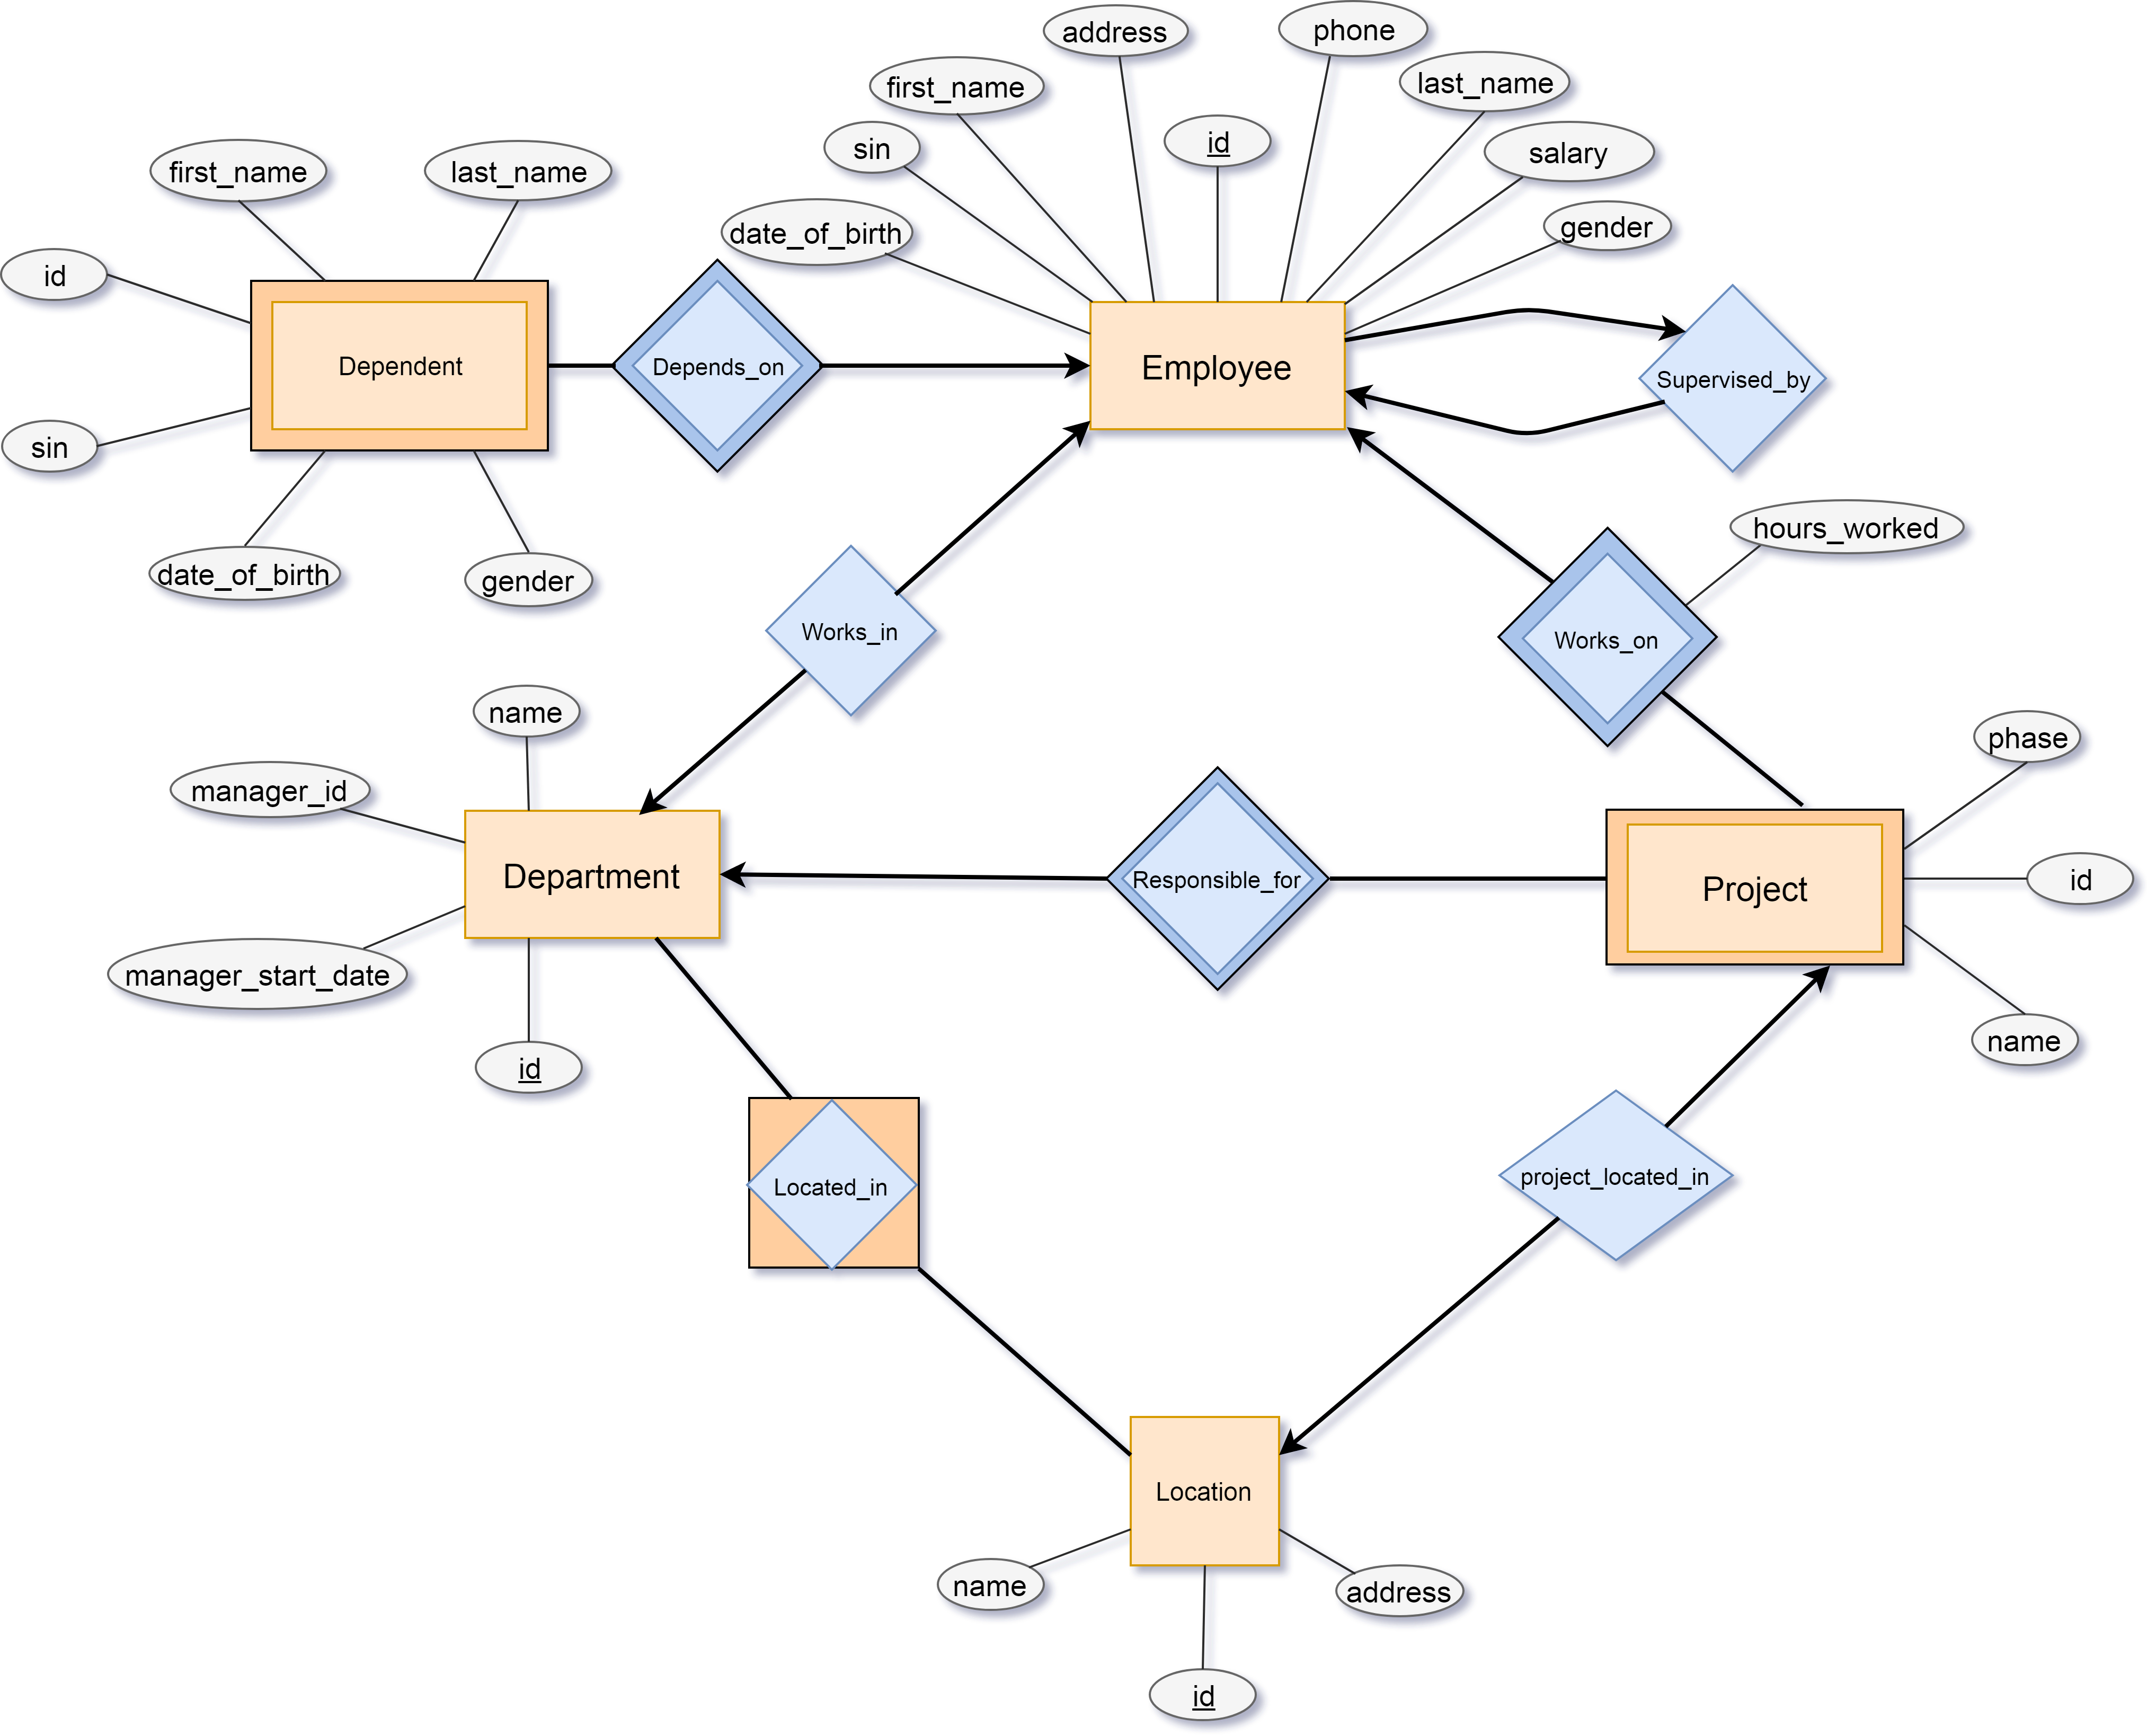
\includegraphics[width=\graphicwidth]{erd.png}
	\section{Reasonable Assumptions}
		\subsection{general cases}
	An assumption is made that all identification numbers are unsigned integers. An \uline{identification key} will never have a sign so the database restricts this. \\	
	
	\subsection{department table}
	In the case of the `department` table, both the \uline{manager\_id} and \uline{manager\_start\_date} are given the opportunity to be null since it is not always true that a `department` needs a manager. Small groups could potentially self manage if that is the policy of the company. \\
	\subsection{employee table}
	To ensure there will always be relevant `employee` data, there are no optional or null possible parameters possible within the `employee`  table. It is assumed that a company needs to keep accurate track of everyone within it and null values would encourage poor data management practice of the company. A \uline{salary}(a 5,2 decimal datatype) is given to each employee in dollars per hour to make certain queries easier to process. Due to legislation, \uline{gender} attribute is defined by one ambiguous character. An `employee` must work for a single `department`.\\
	
		\subsection{project table}
	 It is assumed that a `project` can not be assigned to multiple `departments`. Also a `project` has a varchar \uline{phase} attribute which keeps track of the progress of each individual project within the COMPANY database.\\

		\subsection{dependent table}
The `dependent` table holds vital information that has potential legal importance so none of these fields may be null. A dependent is linked to an `employee` by a foreign key holding \uline{employee\_id} and has the multiplicity of one to many. An `employee` may have many `dependents`. \\

\subsection{location table}
In order to specify where a `project` or `department` is situated, a `location` table keeps track of all of the possible locations where departments and projects operate. An entity table will therefore use a relation table holding an unsigned \uline{location\_id} to specify where the department or project is located in both address and an optional name. The \uline{name} is assumed to be used for employee convenience to identify a location while a mandatory \uline{address} is used for more direct positioning and referencing(as would be used by a post office). The \uline{name} is a varchar, while the \uline{address} is medium text since it is assumed that the address could be as specific as country down to room number and limitations on varchar size could be problematic.\\

\subsection{supervised\_by table}
The `supervised\_by table` defines a role of being a subordinate to someone and helps to give information about the status of an employee in the business hierarchy. Supervision does not imply that an employee is a manager and it could be that an employee both supervises and manages a `department`. It is assumed that this relation is solely used to show the hierarchy of employees within the company. To recognize the `employee` who is supervised, each employee is given a single \uline{supervisor\_id} with a 1:1 multiplicity. Our assumption is that an employee should only be supervised by one person or none at all therefore \uline{employee \_id} is a primary key enforcing uniqueness while \uline{supervisor\_id} is a default null value, where null implies an `employee` is unsupervised.\\

\subsection{depends\_on relation}
	The weak relation  `depends\_on` creates the assumption an `employee` can have many `dependants` in a 1:many relationship.
	
\subsection{works\_on relation}
	The weak relation `works\_on` creates the assumption that an `employee` can work on many `projects` in a 1:many relationship
\subsection{works\_in relation}
The strong relation `works\_in` creates the assumption that an `employee` can only work in one `department` in a 1:1 relationship.
\subsection{responsible\_for relation}
	The weak relation `responsible\_for` creates the assumption that a `department` can be responsible for many `projects` in a 1:many relationship
\subsection{project\_located\_in relation}
The strong relation `project\_located\_in` creates the assumption that a project has to be tied to one location in a 1:1 relationship.
\subsection{department\_located\_in relation}
The associative entity `project\_located\_in` creates the assumption that a `department` can be positioned in many `locations` while at the same time a `location` can be assigned to many `departments` in a many:many relationship.

\pagebreak

\section{ER to Relation conversion }

\pagebreak

\section {Normalization steps and assumptions}

\pagebreak

\section{Implemented Functionalities}
\subsection{Database design}
In the COMPANY database There are three primary categories of entity from which more complex entities are defined. These are:
\begin{enumerate}[]
	\item departments, 
	\item employees,
	\item projects,
\end{enumerate}
Each of these tables specifies information that defines the three main entities in the database. These three main entity sets are also enhanced by the entity sets of:
\begin{enumerate}[]
	\item dependent 
	\item location	
\end{enumerate}	
And also the role relation:
\begin{enumerate}[]	
	\item supervised\_by 	
\end{enumerate}
Which specifies an employees role against other employees as a supervisor.\\
While the entity-relation diagram specifies multiple that multiple possible relations can be made, in order to reduce the complexity of the design(and therefore the queries) only the following relations are used
\begin{enumerate}[]
	\item works\_on
	\item responsible\_for
	\item located\_in
\end{enumerate}
These three relations were deemed most important and the other relations seen on the E/R diagram have been omitted.

\subsection{Language and tools}
	The application makes use of the PHP 5.5.9 language due to it's reliable and simple functions for connecting with a MySQL database. In order to more easily input queries on the database and build a modern looking front end system, Laravel has been used to make development easier which adds additional functionality to and shortcuts to front-end design.\\

\subsection{Query Functionalities}
	Queries allow the system to select, update, modify and add to the company database whilst also providing key information. All of these queries can be found in /laravel/app/http/routes.php while some can also be found in the .php files found in /queries - forms. The \textit{?} and \textit{:id} fields are instances where a dynamic value would be inserted by the Laravel controllers that have been implemented. These dynamic values are captured from a user's input.
	\subsubsection{Department}
	\begin{enumerate}
		\item Select a single department\\ SELECT * \\FROM department \\WHERE id = :id;
		\item Select all departments \\SELECT * \\FROM department \\ORDER BY id;
		\item Select a department's locations\\SELECT * \\FROM located\_in, location \\ WHERE location\_id = id AND department\_id = :id;
		\item Select a department's projects \\SELECT *\\ FROM responsible\_for, project \\WHERE project\_id = id AND department\_id = :id\\ ORDER BY project\_id;
		\item Select all employees for a department \\SELECT * \\FROM employee \\WHERE department\_id = :id \\ORDER BY last\_name;
		\item Select a department's total pay as a function of employee's salary and hours worked\\SELECT SUM(salary * hours\_worked) as 'Pay', department\_id \\FROM works\_on, employee, project \\WHERE employee\_id = employee.id AND project\_id = project.id AND department\_id=:id \\GROUP BY department\_id;
		\item Select locations that a department is not in\\SELECT * \\FROM location \\WHERE id NOT IN (SELECT location\_id FROM located\_in WHERE department\_id = :id);
		\item Add location to a department \\INSERT INTO located\_in(location\_id, department\_id) VALUES (?, ?);
		\item Delete department location \\DELETE FROM located\_in WHERE department\_id = ? AND location\_id = ?; 
		\item Delete a project from department \\DELETE FROM responsible\_for WHERE department\_id = ? AND project\_id = ?;
		\item Select projects without a department \\SELECT * \\FROM project \\WHERE id NOT IN (SELECT project\_id FROM responsible\_for);
		\item Add project to a department\\INSERT INTO responsible\_for(department\_id, project\_id) VALUES (?, ?);
		\item Create a deaprtment\\INSERT INTO department(name, manager\_id, manager\_start\_date) VALUES (?, ?, ?);
		\item Edit a department \\UPDATE department SET name = ?, manager\_id = ?, manager\_start\_date = ? WHERE id = ?;
		\item Delete a department \\DELETE FROM department WHERE id = :id;
	\end{enumerate}

	\subsubsection{Employee}
	\begin{enumerate}
		\item Select a single employee \\SELECT * \\FROM employee \\WHERE id = :id;
		\item Select all employees \\SELECT * \\FROM employee \\ORDER BY id;
		\item Select an employee's dependents\\SELECT * \\FROM dependent \\WHERE employee\_id = :id \\ORDER BY last\_name;
		\item Select projects that an employee works on\\SELECT * \\FROM project, works\_on \\WHERE id = works\_on.project\_id AND works\_on.employee\_id = :id;
		\item Create an employee \\INSERT INTO employee (first\_name, last\_name, sin, date\_of\_birth, address, phone, salary, gender, department\_id) VALUES (?, ?, ?, ?, ?, ?, ?, ?, ?);
		\item Edit an employee \\UPDATE employee SET first\_name = ?, last\_name = ?, sin = ?, date\_of\_birth = ?, address = ?, phone = ?, salary = ?, gender = ?, department\_id = ? WHERE id = ?;
		\item Delete an employee\\DELETE FROM employee WHERE id = :id;
		\item Select all dependents \\SELECT * FROM dependent WHERE id = :id;
		\item Create a dependent \\INSERT INTO dependent(first\_name, last\_name, sin, date\_of\_birth, gender, employee\_id) VALUES (?, ?, ?, ?, ?, ?);
		\item Edit a dependent \\UPDATE dependent SET first\_name = ?, last\_name = ?, sin = ?, date\_of\_birth = ?, gender = ? WHERE id = ?;
		\item Delete a dependent \\DELETE FROM dependent WHERE id = :id;
	\end{enumerate}

	\subsubsection{Supervisor}
	\begin{enumerate}
		\item Select an employee's supervisor\\SELECT * \\FROM role, employee \\WHERE employee.id = supervisor\_id AND employee\_id = :id;
		\item Select a supervisor's subordinates \\SELECT * \\FROM employee \\WHERE id IN (SELECT employee\_id FROM role WHERE supervisor\_id = :id);
		\item Select employees that are not supervisors \\SELECT * \\FROM employee \\WHERE id NOT IN (SELECT supervisor\_id FROM role) \\ORDER BY last\_name;
		\item Select all supervisors \\SELECT * \\FROM employee \\WHERE id IN (SELECT supervisor\_id FROM role);
		\item Select a supervisor\\SELECT * \\FROM employee \\WHERE id = (SELECT DISTINCT supervisor\_id FROM role WHERE supervisor\_id = :id);
		\item Create a supervisor \\INSERT INTO role(employee\_id, supervisor\_id) VALUES (?, ?);
		\item Select employees without supervisors SELECT * FROM employee WHERE id NOT IN (SELECT employee\_id FROM role) AND id $<$$>$ :id;
		\item Delete a subordinate \\DELETE FROM role WHERE employee\_id = ? AND supervisor\_id = ?;
		\item Delete a supervisor \\DELETE FROM role WHERE supervisor\_id = :id;
	\end{enumerate}

	\subsubsection{Projects}
	\begin{enumerate}
		\item Select all projects \\SELECT * \\FROM project \\ORDER BY id;
		\item Select a single project \\SELECT * \\FROM project \\WHERE id = :id;
		\item Select a project's department \\SELECT * \\FROM responsible\_for, department \\WHERE department\_id = id AND project\_id = :id;
		\item Select all employees for a project \\SELECT * \\FROM works\_on, employee \\WHERE id = employee\_id AND project\_id = :id \\ORDER BY id;
		\item Select number of employees for a given project \\SELECT COUNT(id) \\FROM works\_on, employee \\WHERE id = employee\_id AND project\_id = :id;
		\item Select total number of hours worked on a project \\SELECT SUM(hours\_worked) \\FROM works\_on, employee \\WHERE id = employee\_id AND project\_id = :id;
		\item Select a project's total pay \\SELECT SUM(Pay) \\FROM (SELECT works\_on.hours\_worked, works\_on.employee\_id, employee.salary, (hours\_worked * salary) AS Pay \\FROM works\_on, employee \\WHERE  works\_on.project\_id=:id AND employee.id=works\_on.employee\_id) as Payed; 
		\item Create a project \\INSERT INTO project(name, location\_id, phase) VALUES (?, ?, ?);
		\item Edit a project \\UPDATE project SET name = ?, location\_id = ?, phase = ? WHERE id = ?; 
		\item Delete a project \\DELETE FROM project WHERE id = :id;
		\item Select employees not assigned to a project \\SELECT * \\FROM employee \\WHERE id NOT IN (SELECT employee\_id FROM works\_on);
		\item Add an employee to a project \\INSERT INTO works\_on(project\_id, employee\_id, hours\_worked) VALUES (?, ?, ?);
		\item Select an employee working on a project \\SELECT * \\FROM works\_on \\WHERE employee\_id = :eid AND project\_id = :id;
		\item Edit an employee who is working on a project \\UPDATE works\_on SET hours\_worked = ? WHERE employee\_id = ? AND project\_id = ?; 
		\item Delete an employee from a project \\DELETE FROM works\_on WHERE employee\_id = :eid AND project\_id = :id;
	\end{enumerate}

	\subsubsection{Location}
	\begin{enumerate}
		\item Select a single location \\SELECT * \\FROM location \\WHERE id = :id;
		\item Select all locations \\SELECT * \\FROM location \\ORDER BY id;
		\item Select a location's departments \\SELECT * \\FROM department \\WHERE id IN (SELECT department\_id FROM located\_in WHERE location\_id = :id);
		\item Select a location's projects \\SELECT * \\FROM project \\WHERE id IN (SELECT project\_id FROM responsible\_for WHERE department\_id IN (SELECT department\_id FROM located\_in WHERE location\_id = :id)) AND location\_id = :id2;
		\item Create a location \\INSERT INTO location(name, address) VALUES (?, ?); 
		\item Edit a location \\UPDATE location SET name = ?, address = ? WHERE id = ?;
		\item Delete a location \\DELETE FROM location WHERE id = :id;
	\end{enumerate}

	\subsubsection{Statistics}
	\begin{enumerate}
		\item Select count of departments \\SELECT COUNT(id) \\FROM department;
		\item Select count of employees \\SELECT COUNT(id) \\FROM employee;
		\item Select count of projects \\SELECT COUNT(id) \\FROM project; 
		\item Select count of locations \\SELECT COUNT(id) \\FROM location;
		\item Select department with the most employees \\SELECT COUNT(department\_id) as 'Count', department\_id \\FROM employee \\GROUP BY department\_id \\ORDER BY COUNT(department\_id) DESC LIMIT 1;
		\item Select department with the least employees \\SELECT COUNT(department\_id) as 'Count', department\_id \\FROM employee \\GROUP BY department\_id \\ORDER BY COUNT(department\_id) ASC LIMIT 1;
	\pagebreak
		\item Select department with the most projects \\SELECT COUNT(project\_id) as 'Count', department\_id \\FROM responsible\_for \\GROUP BY department\_id \\ORDER BY COUNT(department\_id) DESC LIMIT 1;
		\item Select department with the least projects \\SELECT COUNT(project\_id) as 'Count', department\_id \\FROM responsible\_for \\GROUP BY department\_id \\ORDER BY COUNT(department\_id) ASC LIMIT 1;
		\item Select department with the highest pay \\SELECT SUM(salary * hours\_worked) as 'Pay', department\_id \\FROM works\_on, employee, project \\WHERE employee\_id = employee.id AND project\_id = project.id \\GROUP BY department\_id \\ORDER BY SUM(salary * hours\_worked) DESC LIMIT 1;
		\item Select department with the lowest pay \\SELECT SUM(salary * hours\_worked) as 'Pay', department\_id \\FROM works\_on, employee, project \\WHERE employee\_id = employee.id AND project\_id = project.id \\GROUP BY department\_id \\ORDER BY SUM(salary * hours\_worked) ASC LIMIT 1;
		\item Select project with the highest pay \\SELECT project\_id, project.name, SUM(salary * hours\_worked) as 'Pay' \\FROM works\_on, employee, project \\WHERE employee\_id = employee.id AND project\_id = project.id \\GROUP BY project\_id \\ORDER BY SUM(salary * hours\_worked) DESC LIMIT 1;
		\item Select project with the lowest pay \\SELECT project\_id, project.name, SUM(salary * hours\_worked) as 'Pay' \\FROM works\_on, employee, project \\WHERE employee\_id = employee.id AND project\_id = project.id \\GROUP BY project\_id \\ORDER BY SUM(salary * hours\_worked) ASC LIMIT 1;
		\item Select project with the most employees \\SELECT project\_id, COUNT(employee\_id) as 'Count', project.name \\FROM works\_on, project \\WHERE project\_id = project.id \\GROUP BY project\_id \\ORDER BY COUNT(employee\_id) DESC LIMIT 1;
		\item Select project with the least employees \\SELECT project\_id, COUNT(employee\_id) as 'Count', project.name \\FROM works\_on, project \\WHERE project\_id = project.id \\GROUP BY project\_id \\ORDER BY COUNT(employee\_id) ASC LIMIT 1;
	\pagebreak
		\item Select the total pay for the whole company \\SELECT SUM(Pay) \\FROM (SELECT project\_id, project.name, SUM(salary * hours\_worked) as Pay \\FROM works\_on, employee, project \\WHERE employee\_id = employee.id AND project\_id = project.id \\GROUP BY project\_id) AS P;
		\item Select the company's weekly pay \\SELECT SUM(40*department\_cost\_per\_hour) AS Pay \\FROM department\_cost;\\ \\ ** This query is based off a custom view built on the database ** \\ \\ View creation: \\ CREATE VIEW department\_cost AS\\ SELECT department\_id, SUM(salary) AS department\_cost\_per\_hour \\FROM department,employee \\WHERE 									department.id=employee.department\_id \\GROUP BY department\_id;
		\item Select total project hours \\SELECT SUM(hours\_worked) as 'Count' \\FROM works\_on; total project hours;
		\item Select employee with the most projects \\SELECT COUNT(project\_id) as 'Count', works\_on.employee\_id, employee.first\_name, employee.last\_name \\FROM works\_on \\JOIN employee ON employee.id=works\_on.employee\_id \\GROUP BY employee\_id \\ORDER BY COUNT(project\_id) DESC LIMIT 1;
		\item Select employee with the least projects \\SELECT COUNT(project\_id) as 'Count', works\_on.employee\_id, employee.first\_name, employee.last\_name \\FROM works\_on \\JOIN employee ON employee.id=works\_on.employee\_id \\GROUP BY employee\_id \\ORDER BY COUNT(project\_id) ASC LIMIT 1;
		\item Select supervisor with the most subordinates \\SELECT COUNT(employee\_id) as 'Count', supervisor\_id, first\_name, last\_name \\FROM role, employee \\WHERE supervisor\_id = id \\GROUP BY supervisor\_id \\ORDER BY COUNT(employee\_id) DESC LIMIT 1;
		\item Select supervisor with the least subordinates \\SELECT COUNT(employee\_id) as 'Count', supervisor\_id, first\_name, last\_name \\FROM role, employee \\WHERE supervisor\_id = id \\GROUP BY supervisor\_id \\ORDER BY COUNT(employee\_id) ASC LIMIT 1;
		\item Select total salary per hour \\SELECT SUM(salary) as 'Count' \\FROM employee;
		\item Select location with the most projects \\SELECT location\_id, location.name, COUNT(project.id) as 'Count' \\FROM project, location \\WHERE project.id IN (SELECT project\_id FROM responsible\_for WHERE department\_id IN (SELECT department\_id FROM located\_in)) AND location\_id = location.id \\GROUP BY location\_id \\ORDER BY COUNT(project.id) DESC LIMIT 1;
		\item Select location with the least projects \\SELECT location\_id, location.name, COUNT(project.id) as 'Count' \\FROM project, location \\WHERE project.id IN (SELECT project\_id FROM responsible\_for WHERE department\_id IN (SELECT department\_id FROM located\_in)) AND location\_id = location.id \\GROUP BY location\_id \\ORDER BY COUNT(project.id) ASC LIMIT 1;
	\end{enumerate}
	
\pagebreak

\section{Contributions}
\subsection{Giovanni Gebran}
 \begin{itemize}
\item Database Design
\item Functional Dependencies
\end{itemize}
\subsection{Nizar Belhassan}
 \begin{itemize}
\item Database Design
\item Query Implementations
\end{itemize}
\subsection{Kai Nicoll-Griffith}
 \begin{itemize}
\item Database Design
\item Database Attribute Refinements
\item Report Setup and LateX entry
\item Report: ER Diagram
\item Report: Constraints and Assumptions
\item Report: Query Functionalities
\end{itemize}
\subsection{Stephen Prizio}
 \begin{itemize}
	\item Database Design
	\item Laravel Application Development
	\item SQL sample data and Database 
	\item Query Implementations
	\item Report: Query Functionalities
\end{itemize}
\end{document}
